\documentclass[11pt,a4paper]{article}
\usepackage[margin=2.5cm]{geometry}
\usepackage{graphicx}
\usepackage{enumitem}
\usepackage{xcolor}
\usepackage{fancyhdr}
\usepackage{titlesec}
\usepackage{multicol}
\usepackage{caption}

\setlength{\columnsep}{2cm}

% Header setup
\pagestyle{fancy}
\fancyhf{}
\fancyhead[C]{Distance Measurement Device - User Guide}
\fancyfoot[C]{\thepage}

% Section formatting
\titleformat{\section}{\large\bfseries\color{blue!70!black}}{\thesection}{1em}{}
\titleformat{\subsection}{\normalsize\bfseries}{\thesubsection}{1em}{}

\begin{document}

\title{\textbf{Distance Measurement Device}\\ \large User Guide}
\author{}
\date{}
\maketitle

\section{Overview}
This device estimates distances using geometric principles with a folding ruler and string setup. Best accuracy is achieved when measuring objects significantly above or below eye level.

\section{Required Equipment}
\begin{itemize}[noitemsep]
    \item Folding ruler - fully extended
    \item Circular string (neck loop)
    \item Long measuring string
    \item Distance measurement software
\end{itemize}

\section{Software Operation}

\subsection{Input Values}
Enter these measurements into the program:
\begin{itemize}[noitemsep]
    \item \textbf{Relative Height}: Vertical offset to target (+ above, - below eye level)
    \item \textbf{Apparent Height}: Ruler reading where target appears
    \item \textbf{Observation Height}: Your measured eye height
\end{itemize}

\subsection{Procedure}
\begin{enumerate}[noitemsep]
    \item Start distance measurement program
    \item Click \textit{"Use the Model"}
    \item Input three measurements
    \item Receive distance estimate
\end{enumerate}

\newpage

\section{Measurement Steps}

\subsection{Step 1: Initial Setup}
\begin{multicols}{2}
    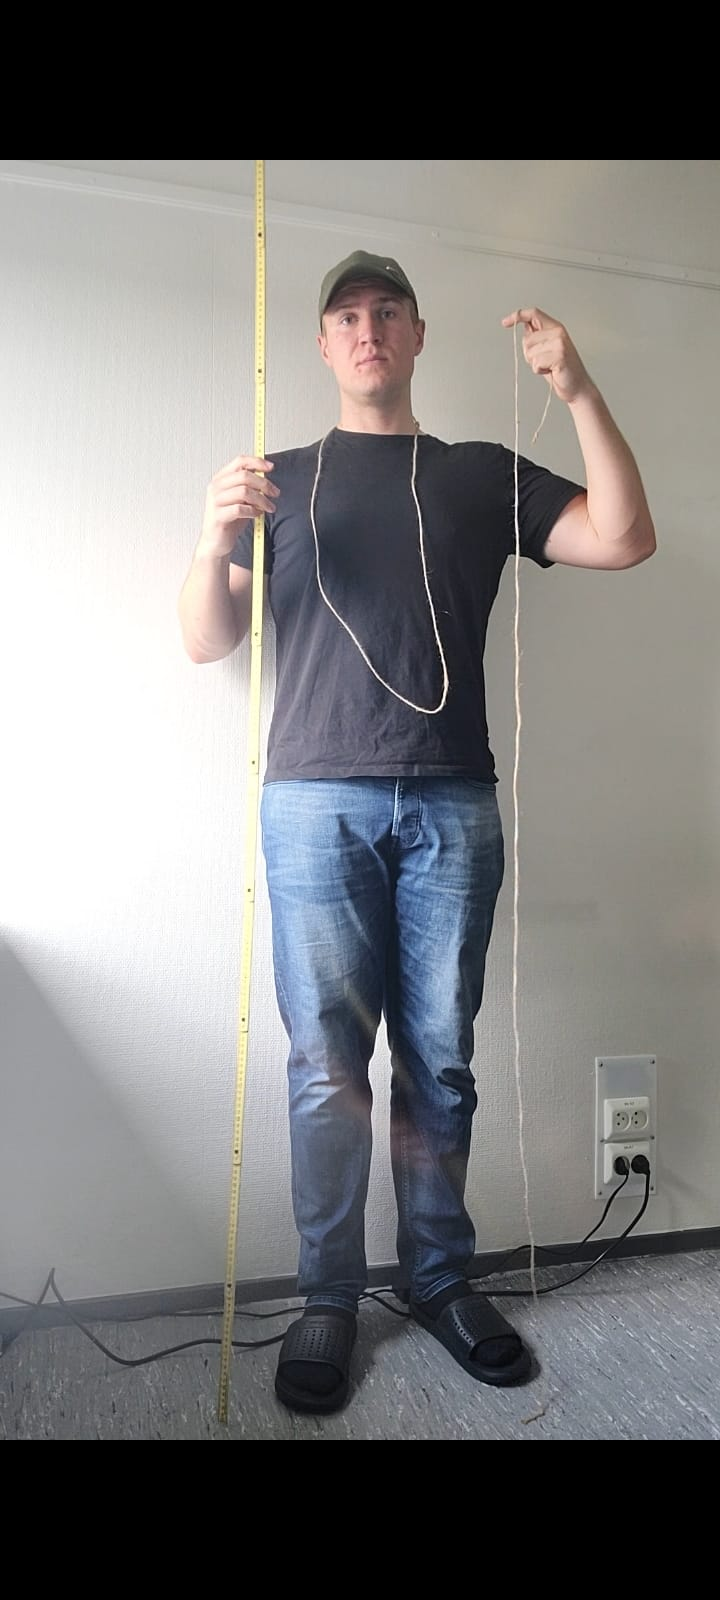
\includegraphics[width=\linewidth]{setup.jpg}
    
    \columnbreak
    
    \begin{enumerate}[noitemsep]
        \item \textbf{Extend} the ruler to full length
        \item \textbf{Place} circular string around your neck
        \item \textbf{Step on} the end of the long string
    \end{enumerate}

    The setup creates the foundation for accurate measurements. Ensure stable footing throughout.
\end{multicols}
\newpage

\subsection{Step 2: Position Measuring Rod}
\begin{multicols}{2}
    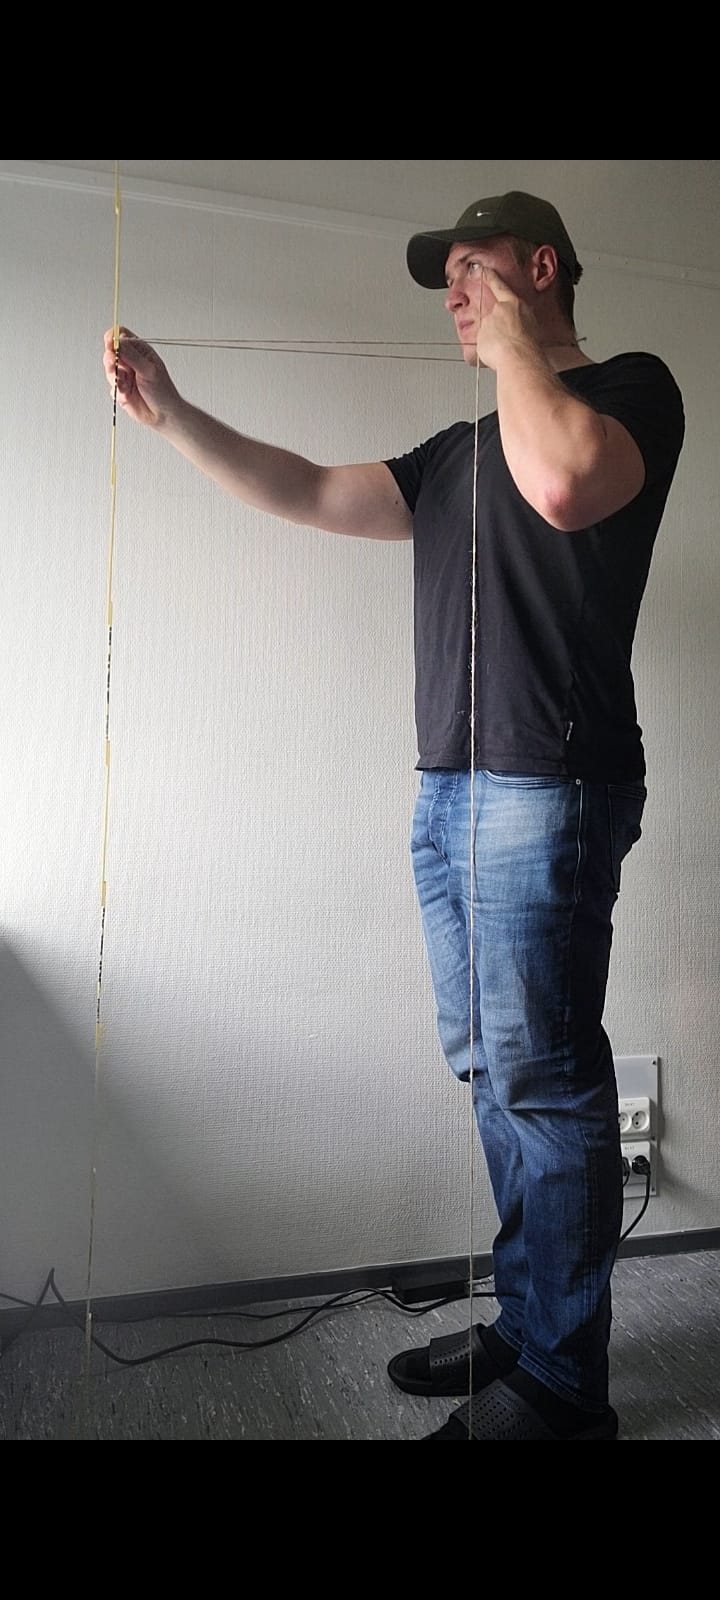
\includegraphics[width=\linewidth]{measure1.jpg}
    
    \columnbreak
    
    \begin{enumerate}[noitemsep]
        \item \textbf{Insert} ruler through neck string
        \item \textbf{Push} ruler away from body as far as possible
        \item \textbf{Let hang} vertically, touching the ground
        \item \textbf{Hold} the foot string at eye level
    \end{enumerate}
    
    Critical: The ruler must hang perfectly vertical for accurate readings.
\end{multicols}
\newpage

\subsection{Step 3: Target Object Measurement}
\begin{multicols}{2}
    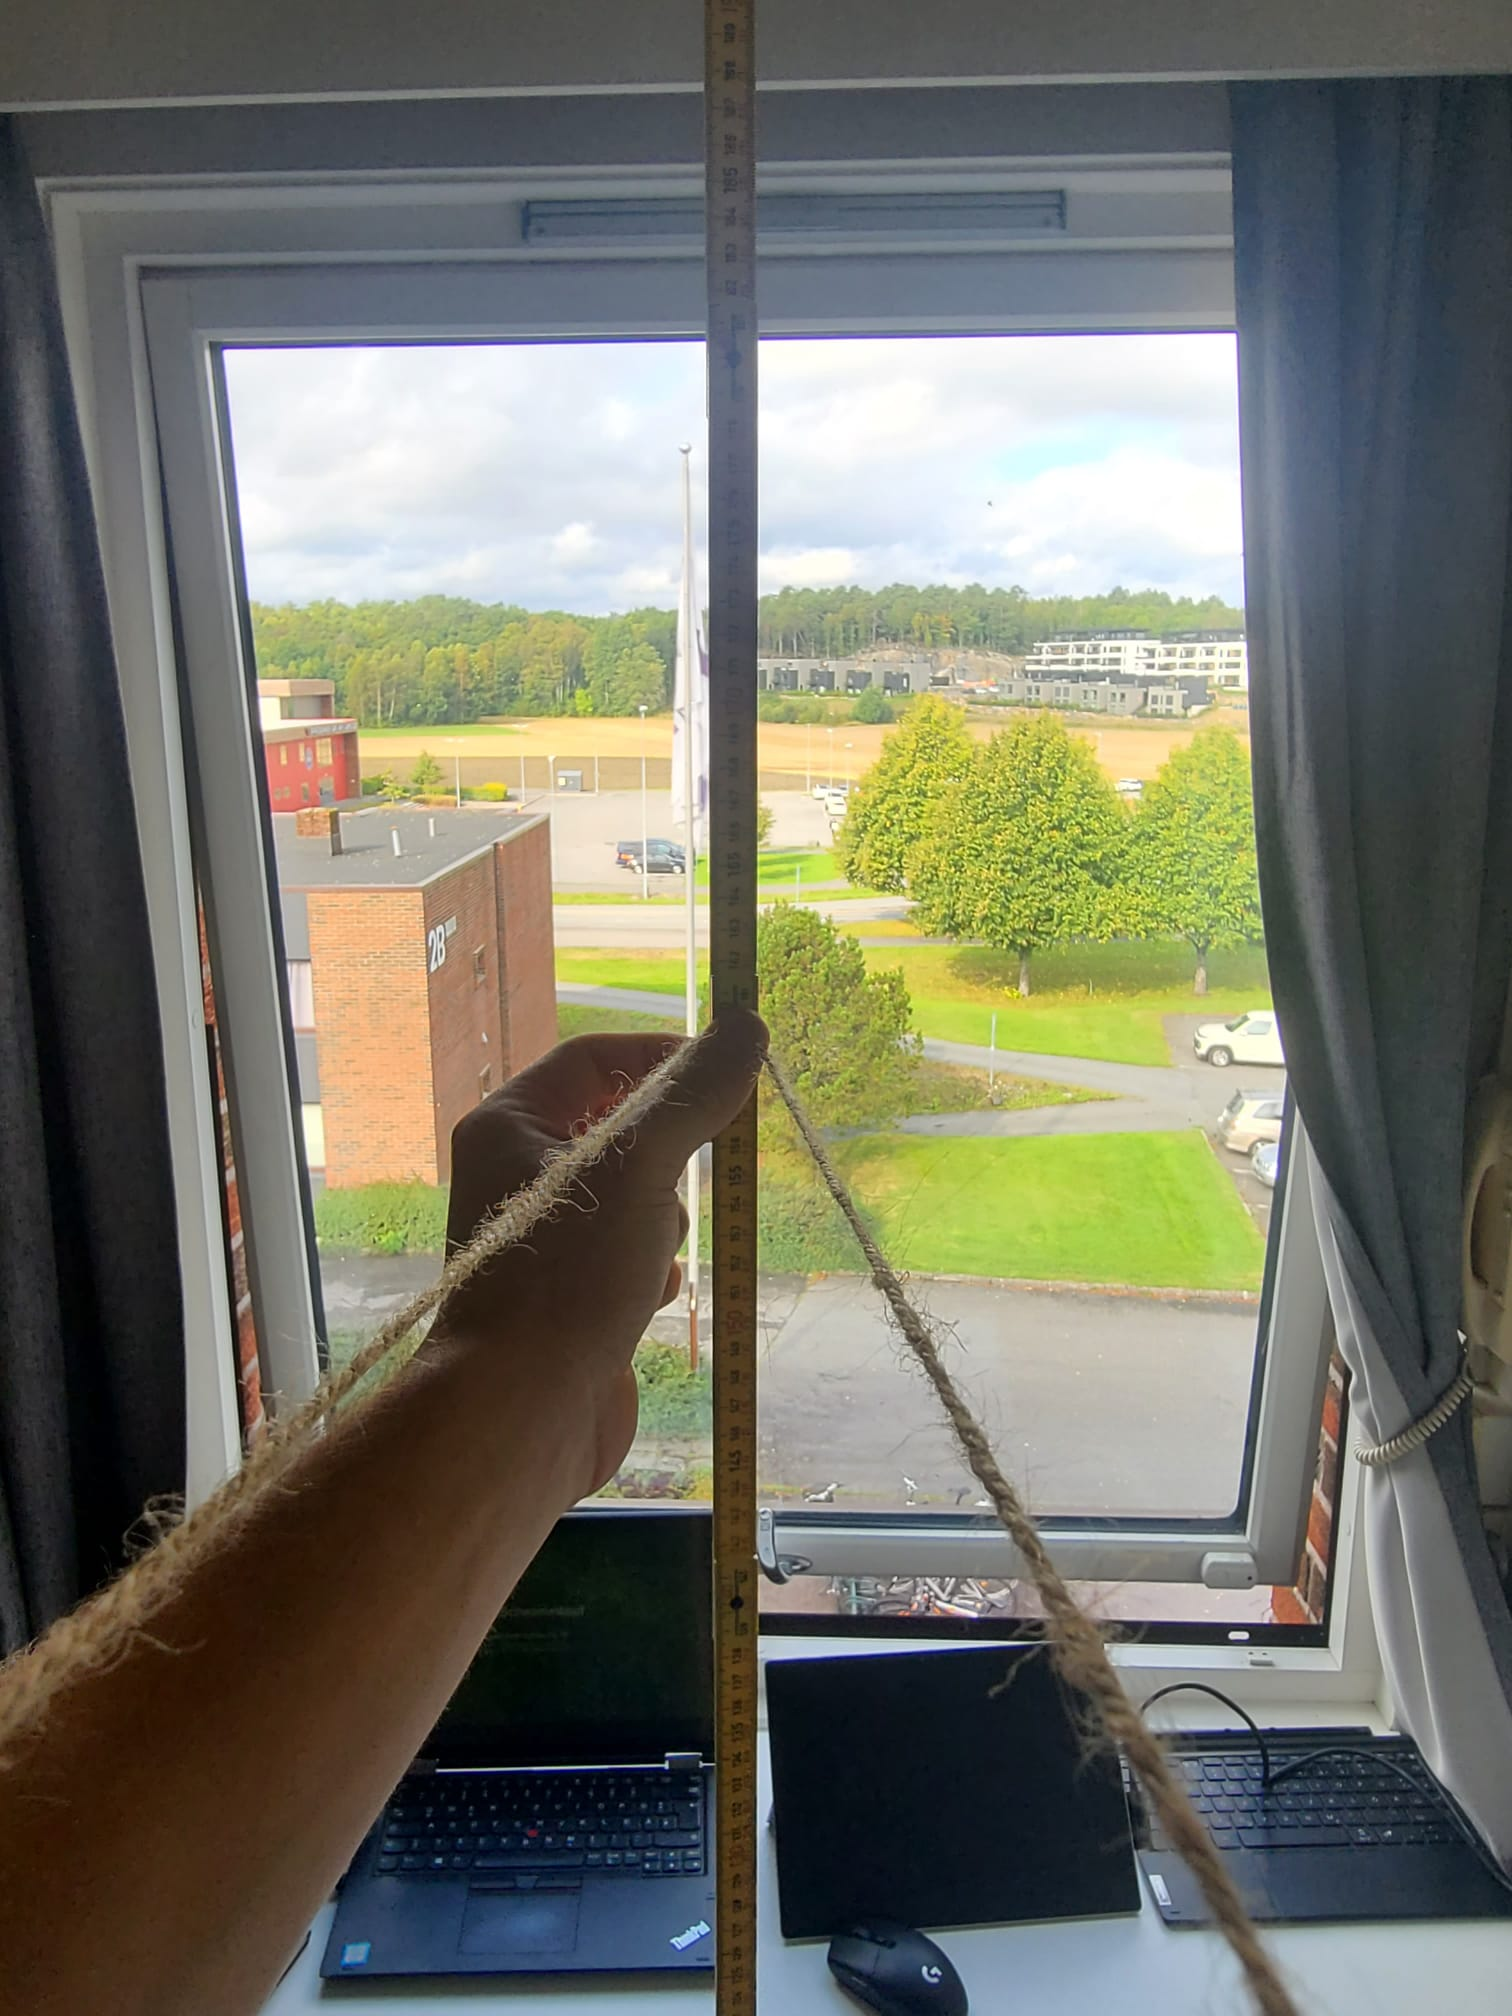
\includegraphics[width=\linewidth]{pov.jpg}
    
    \columnbreak
    
    \begin{enumerate}[noitemsep]
        \item \textbf{Locate} your target object
        \item \textbf{Choose} optimal angle: far above/below eye level
        \item \textbf{Sight} the target along the ruler
        \item \textbf{Read} height marking where target appears
    \end{enumerate}
    
    \textbf{Tip:} For trees, aim for tip or base - choose the larger vertical offset from eye level.
\end{multicols}
\newpage

\subsection{Step 4: Eye Height Measurement}
\begin{multicols}{2}
    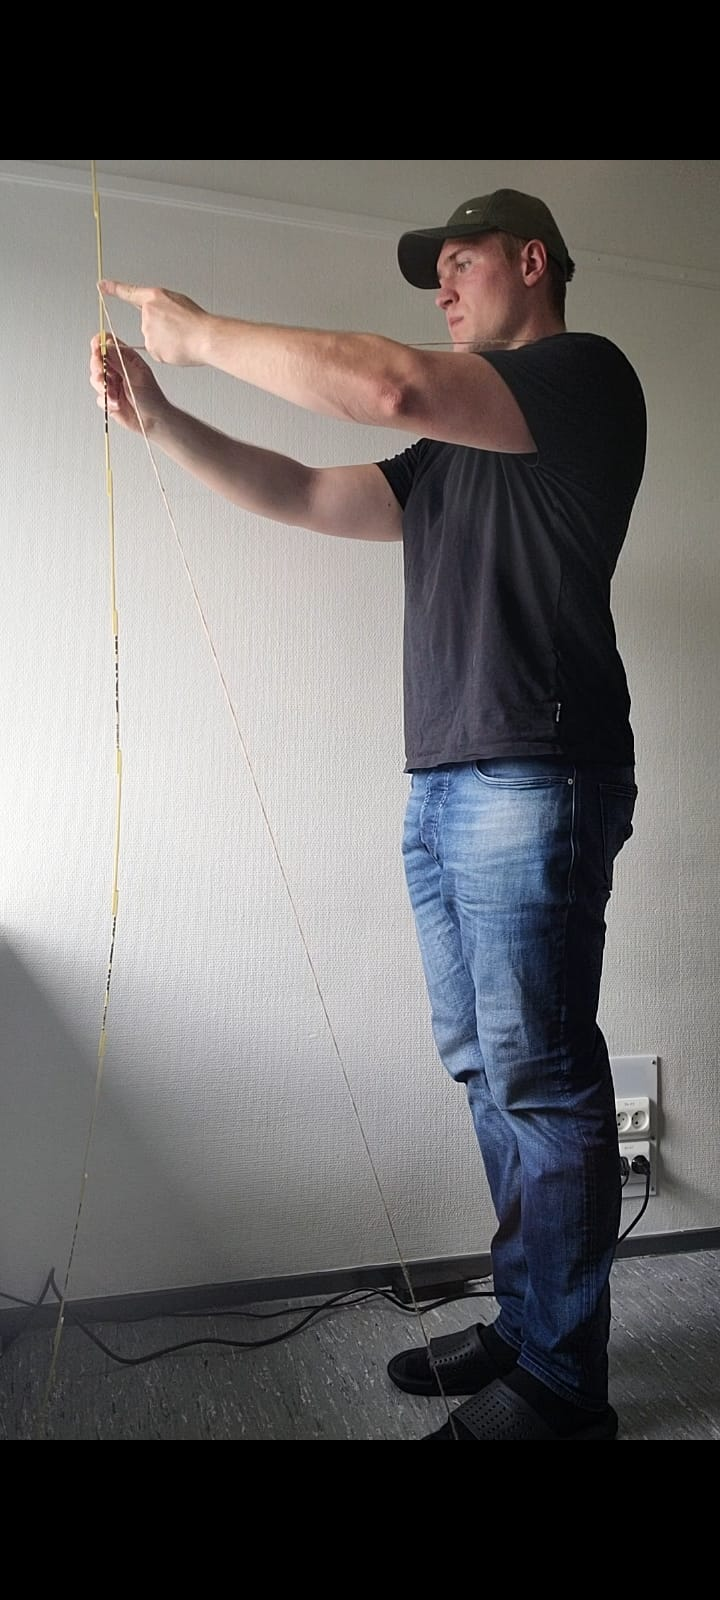
\includegraphics[width=\linewidth]{measure2.jpg}
    
    \columnbreak
    
    \begin{enumerate}[noitemsep]
        \item \textbf{Maintain} string position at eye level
        \item \textbf{Measure} string length on ruler
        \item \textbf{Keep foot} on string end throughout
    \end{enumerate}
    
    This measurement determines your observation height - essential for accurate calculations.
\end{multicols}
\newpage    

\section{Best Practices \& Common Errors}

\begin{multicols}{2}
    \textbf{Optimal Conditions:}
    \begin{itemize}[noitemsep]
        \item Target far above/below eye level
        \item Clear line of sight
        \item Stable, windless conditions
        \item Consistent string tension
    \end{itemize}
    
    \columnbreak
    
    \textbf{Common Errors:}
    \begin{itemize}[noitemsep]
        \item Non-vertical ruler position
        \item Moving between measurements
        \item Ignoring vertical target offset
        \item Inconsistent string handling
    \end{itemize}
\end{multicols}

\vspace{0.5cm}
\textbf{Technical Notes:} Uses similar triangles and machine learning corrections. Results are approximations - verify when precision is critical.

\vspace{0.5cm}
\hrule
\vspace{0.3cm}
\textit{For technical details, refer to distance.py source code.}

\end{document}